% Options for packages loaded elsewhere
\PassOptionsToPackage{unicode}{hyperref}
\PassOptionsToPackage{hyphens}{url}
\PassOptionsToPackage{dvipsnames,svgnames,x11names}{xcolor}
%
\documentclass[
]{interact}

\usepackage{amsmath,amssymb}
\usepackage{iftex}
\ifPDFTeX
  \usepackage[T1]{fontenc}
  \usepackage[utf8]{inputenc}
  \usepackage{textcomp} % provide euro and other symbols
\else % if luatex or xetex
  \usepackage{unicode-math}
  \defaultfontfeatures{Scale=MatchLowercase}
  \defaultfontfeatures[\rmfamily]{Ligatures=TeX,Scale=1}
\fi
\usepackage{lmodern}
\ifPDFTeX\else  
    % xetex/luatex font selection
\fi
% Use upquote if available, for straight quotes in verbatim environments
\IfFileExists{upquote.sty}{\usepackage{upquote}}{}
\IfFileExists{microtype.sty}{% use microtype if available
  \usepackage[]{microtype}
  \UseMicrotypeSet[protrusion]{basicmath} % disable protrusion for tt fonts
}{}
\makeatletter
\@ifundefined{KOMAClassName}{% if non-KOMA class
  \IfFileExists{parskip.sty}{%
    \usepackage{parskip}
  }{% else
    \setlength{\parindent}{0pt}
    \setlength{\parskip}{6pt plus 2pt minus 1pt}}
}{% if KOMA class
  \KOMAoptions{parskip=half}}
\makeatother
\usepackage{xcolor}
\setlength{\emergencystretch}{3em} % prevent overfull lines
\setcounter{secnumdepth}{5}
% Make \paragraph and \subparagraph free-standing
\ifx\paragraph\undefined\else
  \let\oldparagraph\paragraph
  \renewcommand{\paragraph}[1]{\oldparagraph{#1}\mbox{}}
\fi
\ifx\subparagraph\undefined\else
  \let\oldsubparagraph\subparagraph
  \renewcommand{\subparagraph}[1]{\oldsubparagraph{#1}\mbox{}}
\fi


\providecommand{\tightlist}{%
  \setlength{\itemsep}{0pt}\setlength{\parskip}{0pt}}\usepackage{longtable,booktabs,array}
\usepackage{calc} % for calculating minipage widths
% Correct order of tables after \paragraph or \subparagraph
\usepackage{etoolbox}
\makeatletter
\patchcmd\longtable{\par}{\if@noskipsec\mbox{}\fi\par}{}{}
\makeatother
% Allow footnotes in longtable head/foot
\IfFileExists{footnotehyper.sty}{\usepackage{footnotehyper}}{\usepackage{footnote}}
\makesavenoteenv{longtable}
\usepackage{graphicx}
\makeatletter
\def\maxwidth{\ifdim\Gin@nat@width>\linewidth\linewidth\else\Gin@nat@width\fi}
\def\maxheight{\ifdim\Gin@nat@height>\textheight\textheight\else\Gin@nat@height\fi}
\makeatother
% Scale images if necessary, so that they will not overflow the page
% margins by default, and it is still possible to overwrite the defaults
% using explicit options in \includegraphics[width, height, ...]{}
\setkeys{Gin}{width=\maxwidth,height=\maxheight,keepaspectratio}
% Set default figure placement to htbp
\makeatletter
\def\fps@figure{htbp}
\makeatother
\newlength{\cslhangindent}
\setlength{\cslhangindent}{1.5em}
\newlength{\csllabelwidth}
\setlength{\csllabelwidth}{3em}
\newlength{\cslentryspacingunit} % times entry-spacing
\setlength{\cslentryspacingunit}{\parskip}
\newenvironment{CSLReferences}[2] % #1 hanging-ident, #2 entry spacing
 {% don't indent paragraphs
  \setlength{\parindent}{0pt}
  % turn on hanging indent if param 1 is 1
  \ifodd #1
  \let\oldpar\par
  \def\par{\hangindent=\cslhangindent\oldpar}
  \fi
  % set entry spacing
  \setlength{\parskip}{#2\cslentryspacingunit}
 }%
 {}
\usepackage{calc}
\newcommand{\CSLBlock}[1]{#1\hfill\break}
\newcommand{\CSLLeftMargin}[1]{\parbox[t]{\csllabelwidth}{#1}}
\newcommand{\CSLRightInline}[1]{\parbox[t]{\linewidth - \csllabelwidth}{#1}\break}
\newcommand{\CSLIndent}[1]{\hspace{\cslhangindent}#1}

\usepackage{orcidlink}
\usepackage{tikz}
\usetikzlibrary{positioning}
\makeatletter
\@ifpackageloaded{tikz}{}{\usepackage{tikz}}
\makeatother
\makeatletter
\makeatother
\makeatletter
\@ifpackageloaded{caption}{}{\usepackage{caption}}
\AtBeginDocument{%
\ifdefined\contentsname
  \renewcommand*\contentsname{Table of contents}
\else
  \newcommand\contentsname{Table of contents}
\fi
\ifdefined\listfigurename
  \renewcommand*\listfigurename{List of Figures}
\else
  \newcommand\listfigurename{List of Figures}
\fi
\ifdefined\listtablename
  \renewcommand*\listtablename{List of Tables}
\else
  \newcommand\listtablename{List of Tables}
\fi
\ifdefined\figurename
  \renewcommand*\figurename{Figure}
\else
  \newcommand\figurename{Figure}
\fi
\ifdefined\tablename
  \renewcommand*\tablename{Table}
\else
  \newcommand\tablename{Table}
\fi
}
\@ifpackageloaded{float}{}{\usepackage{float}}
\floatstyle{ruled}
\@ifundefined{c@chapter}{\newfloat{codelisting}{h}{lop}}{\newfloat{codelisting}{h}{lop}[chapter]}
\floatname{codelisting}{Listing}
\newcommand*\listoflistings{\listof{codelisting}{List of Listings}}
\makeatother
\makeatletter
\@ifpackageloaded{caption}{}{\usepackage{caption}}
\@ifpackageloaded{subcaption}{}{\usepackage{subcaption}}
\makeatother
\makeatletter
\@ifpackageloaded{tcolorbox}{}{\usepackage[skins,breakable]{tcolorbox}}
\makeatother
\makeatletter
\@ifundefined{shadecolor}{\definecolor{shadecolor}{rgb}{.97, .97, .97}}
\makeatother
\makeatletter
\makeatother
\makeatletter
\makeatother
\ifLuaTeX
  \usepackage{selnolig}  % disable illegal ligatures
\fi
\IfFileExists{bookmark.sty}{\usepackage{bookmark}}{\usepackage{hyperref}}
\IfFileExists{xurl.sty}{\usepackage{xurl}}{} % add URL line breaks if available
\urlstyle{same} % disable monospaced font for URLs
\hypersetup{
  pdftitle={Research Report},
  pdfauthor={Pepijn Vink (6100252)},
  pdfkeywords={lorem, ipsum},
  colorlinks=true,
  linkcolor={blue},
  filecolor={Maroon},
  citecolor={Blue},
  urlcolor={Blue},
  pdfcreator={LaTeX via pandoc}}

\title{Research Report}
\author{Pepijn Vink
(6100252)$\textsuperscript{1}$~\orcidlink{0000-0001-6960-9904}}

\thanks{CONTACT: Pepijn Vink
(6100252). Email: \href{mailto:p.a.vink@uu.nl}{\nolinkurl{p.a.vink@uu.nl}}. }
\begin{document}
\captionsetup{labelsep=space}
\maketitle
\textsuperscript{1} Methodology and Statistics for the Behavioral,
Biomedical, and Social Sciences, Utrecht University,  
\begin{abstract}
Lorem Ipsum\ldots{}
\end{abstract}
\begin{keywords}
\def\sep{;\ }
lorem\sep 
ipsum
\end{keywords}
\ifdefined\Shaded\renewenvironment{Shaded}{\begin{tcolorbox}[breakable, enhanced, frame hidden, boxrule=0pt, interior hidden, sharp corners, borderline west={3pt}{0pt}{shadecolor}]}{\end{tcolorbox}}\fi

\newcommand{\indep}{\perp \!\!\! \perp}

\hypertarget{introduction}{%
\section{Introduction}\label{introduction}}

\hypertarget{causal-models-and-backdoor-paths}{%
\subsection{Causal Models and Backdoor
Paths}\label{causal-models-and-backdoor-paths}}

\emph{Include: Introduction to types of DAG structures, backdoor paths,
and terminology}

\hypertarget{confounding-in-cross-lagged-panel-models}{%
\subsection{Confounding in Cross-Lagged Panel
Models}\label{confounding-in-cross-lagged-panel-models}}

\emph{Include: Introduce an example SCM (and possibly the CLPM)}

When taking the effect of \(x_4\) on \(x_5\) as an example, confounding
of this effect happens through several paths. First, there are paths
through the \(x_t\) variables and \(y_t\) variables. An example is the
\(x_4 \leftarrow y_3 \rightarrow y_4 \rightarrow y_5\) path, but also
\(x_4 \leftarrow x_3 \rightarrow y_4 \rightarrow y_5\) and other paths
that go back more. Secondly, there is confounding due to the
time-specific confounders \(U_{it}\). The \(x_4 \rightarrow y_5\) effect
would then be confounded by the
\(x_4 \leftarrow U_4 \rightarrow y_4 \rightarrow y_5\) path (and no
other paths). Lastly, there is confounding through the time-invariant
confounders \(C\). Confounding on the \(x_4 \rightarrow y_5\) path
would, for example be a \(x_4 \leftarrow C_1 \rightarrow y_5\) path, but
also a \(x_4 \leftarrow x_3 \leftarrow C_1 \rightarrow y_5\) and a
\(x_4 \leftarrow x_3 \leftarrow C_1 \rightarrow y_4 \rightarrow y_5\)
path as well as many more. These types of confounding would result in
biased estimates if the coefficient of regressing \(y_5\) on only
\(x_4\) were used as an estimate.

The first type of confounding, confounding through previous instances of
\(x\) and \(y\), can be resolved by controlling for these previous
instances in the regression equation. This is what the classic
cross-lagged panel model does. This also resolves some of the
confounding by \(C\) that runs through previous timepoints of \(x\) and
\(y\), so that the \(x_4 \rightarrow y_5\) path is only confounded by
\(x_4 \leftarrow C \rightarrow y_5\) paths. The second type of
confounding, through time-specific confounders \(U_t\), is resolved by
allowing residuals of \(x_t\) and \(y_t\) to be correlated. The third
type of confounding, that through time-invariant confounders \(C\), can
sometimes be resolved through the inclusion of a latent factor, which is
the approach that the random intercept cross-lagged panel model
(RI-CLPM) and the dynamic panel model (DPM) take.

\hypertarget{comparison-of-ri-clpm-and-dpm}{%
\subsection{Comparison of RI-CLPM and
DPM}\label{comparison-of-ri-clpm-and-dpm}}

\emph{i.e.~residual based and observed based. conceptual
interpretations}

\hypertarget{ri-clpm-and-dpm-as-data-generating-mechanisms}{%
\subsection{RI-CLPM and DPM as Data Generating
Mechanisms}\label{ri-clpm-and-dpm-as-data-generating-mechanisms}}

Although the RI-CLPM and the DPM have some similarities when it comes to
analyses, when interpreting them as causal models each of them has
different implications regarding the data generating mechanism.

The RI-CLPM implies that a person's deviation from their mean at \(t-1\)
has a causal effect on their deviation from their mean at timepoint
\(t\). It implies that the trait-like factor for a time varying variable
\(x\) is only related to the vector of a time varying variable \(y\)
through the covariance with its random intercept. This can reflect, for
example, between person differences in the tendency to give high
responses. It may thus represent a type of measurement error that is
systematic within a person, but random between persons.

The DPM implies that observed scores at timepoint \(t-1\) have a direct
causal effect on observed scores at timepoint \(t\). Furthermore, in the
DPM, the latent factor for \(x\) is allowed to have an effect on
observed scores for \(y\) through the observed scores on \(x\) (and in
part through observed scores in earlier lags of \(y\)), rather than only
through its covariance with the latent factor for \(y\).

\hypertarget{confounding-in-the-ri-clpm-and-dpm}{%
\subsection{Confounding in the RI-CLPM and
DPM}\label{confounding-in-the-ri-clpm-and-dpm}}

It is known that both the RI-CLPM and the DPM, in specific cases,
control for unobserved time-invariant confounders. Usami et al. (2019),
for example, show that when the effects of the confounders are stable
over time, as well as the lagged effects, the confounder does not affect
the estimated of the lagged effects when using the RI-CLPM. The latent
factor in the DPM, however, also controls for time-invariant confounders
with time-invariant effects when lagged effects are not constant over
time (Murayama \& Gfrörer, 2022). Furthermore, estimates will still be
biased when the effects of the confounders are unstable over time.

Therefore, the simplest forms of both the RI-CLPM and the DPM will not
yield unbiased estimates of the causal effects if there are unobserved
time-invariant confounders with time-varying effects. The thesis will
explore ways to address these types of confounding in the RI-CLPM using
causal inference techniques such as propensity score weighting (Brown et
al., 2021; e.g. Vansteelandt \& Daniel, 2014). However, before this
question is answered, the extent to which unobserved time-invariant
confounders affect the estimates of the RI-CLPM and the DPM should be
evaluated. Thus, this research report will explore different types of
time-invariant confounders in panel data (i.e.~with time-stable effects
versus time-varying effects) and assess their effects on estimates of
the RI-CLPM and DPM as well as modified versions of these models with
freed factor loadings.

\hypertarget{methods}{%
\section{Methods}\label{methods}}

\hypertarget{causal-models}{%
\subsection{Causal Models}\label{causal-models}}

For all simulations, the following data generating mechanism will be
simulated:

\begin{equation}\protect\hypertarget{eq-formula-t}{}{
\begin{split}
\begin{bmatrix}
x_{it}\\
y_{it}
\end{bmatrix}
&
=
\boldsymbol{\Phi}\begin{bmatrix}x_{i,t-1}\\y_{i,t-1}\end{bmatrix} + \textbf{B}_{ct}\begin{bmatrix}
C_{1i}\\
C_{2i}
\end{bmatrix} +
U_{it} +
\begin{bmatrix}
\epsilon_{xit}\\
\epsilon_{yit}
\end{bmatrix}\\
&
=
\begin{bmatrix}
\phi_{xx} & \phi_{xy}\\
\phi_{yx} & \phi_{yy}
\end{bmatrix}
\begin{bmatrix}
x_{i,t-1}\\
y_{i,t-1}
\end{bmatrix}
+
\begin{bmatrix}
\beta_{xc_1t} & \beta_{xc_2t}\\
\beta_{yc_1t} & \beta_{yc_2t}
\end{bmatrix}
\begin{bmatrix}
C_{1i}\\
C_{2i}
\end{bmatrix} +
U_{it} +
\begin{bmatrix}
\epsilon_{xit}\\
\epsilon_{yit}
\end{bmatrix}
\end{split}
}\label{eq-formula-t}\end{equation}

for \(t = 2, ..., T\) and

\[
\begin{bmatrix}
x_{i1}\\
y_{i1}
\end{bmatrix}
=
\begin{bmatrix}
\beta_{xc_11} & \beta_{xc_21}\\
\beta_{yc_11} & \beta_{yc_21}
\end{bmatrix}
\begin{bmatrix}
C_{1i}\\
C_{2i}
\end{bmatrix} +
U_{i1} +
\begin{bmatrix}
\epsilon_{xi1}\\
\epsilon_{yi1}
\end{bmatrix}.
\]

Here, for person \(i\) at timepoint \(t\),
\(\begin{bmatrix} x_{it} & y_{it}\end{bmatrix}^T\) is the data vector,
\(\boldsymbol{\Phi}\) is the matrix of lagged effects,
\(\textbf{B}_{ct}\) is the matrix of effects of the time-invariant
confounders, \(\begin{bmatrix} C_{1i} & C_{2i}\end{bmatrix}^T\) is the
vector of confounder values, \(U_{it}\) is the value of the
time-specific confounder, and
\(\begin{bmatrix}\epsilon_{xit} & \epsilon_{yit}\end{bmatrix}^T\) is the
vector of residuals.

In addition,

\[
\begin{bmatrix}
\epsilon_{xit}\\
\epsilon_{yit}
\end{bmatrix}
\sim
\mathcal{N} \left(\begin{bmatrix} 0\\ 0 \end{bmatrix}, \begin{bmatrix} \psi_x & 0\\ 0 & \psi_y \end{bmatrix} \right),
\]

\[
\begin{bmatrix}
C_{1i}\\
C_{2i}
\end{bmatrix} \sim \mathcal{N}\left(\begin{bmatrix} 0\\0 \end{bmatrix}, \begin{bmatrix}\psi_{C_1} & 0 \\0 & \psi_{C_2} \end{bmatrix} \right),
\]

\[
U_{it} \sim \mathcal{N}\left(0, \psi_u\right),
\]

for \(i = 1,..., N\).

This SCM is similar to the DPM as it does not have an explicit
decomposition of within and between effects and it is thus an
observation based model, rather than a residual based model. One way
that it differs from the DPM, other than having an observed confounder
instead of a latent factor, is that the DPM includes covariances between
the residuals at each timepoint. Because our model is specified as a
DAG, two-headed arrows are not included, and this is thus expressed as a
latent confounder between the residuals at each timepoint. It can be
shown that when these the effect of these confounders on the residuals
are 1, this specification using a confounder \(u_t\) with
\(\sigma_{u_t}^2 = \psi_u\) is equivalent to specifying a covariance
between the residuals where \(\sigma_{x_ty_t} = \psi_u\). Furthermore,
the variance of the residuals at each timepoint, \(\psi_x\) and
\(\psi_y\) are equal to the residual variances in the DPM, minus the
variance of the unique factor \(u_t\) at that timepoint.

The specific SCMs that will be simulated are described below.

\hypertarget{one-confounder-time-stable-effects.-model-1}{%
\subsubsection{One confounder, time-stable effects. (Model
1)}\label{one-confounder-time-stable-effects.-model-1}}

When there is only one confounder C, and its effects are invariant over
time, Equation~\ref{eq-formula-t} reduces to:

\[
\begin{bmatrix}
x_{it}\\
y_{it}
\end{bmatrix}
=
\begin{bmatrix}
\phi_{xx} & \phi_{xy}\\
\phi_{yx} & \phi_{yy}
\end{bmatrix}
\begin{bmatrix}
x_{i,t-1}\\
y_{i,t-1}
\end{bmatrix}
+
\begin{bmatrix}
\beta_{xc}\\
\beta_{yc}
\end{bmatrix}
C_{i} +
U_{it} +
\begin{bmatrix}
\epsilon_{xit}\\
\epsilon_{yit}
\end{bmatrix}.
\]

The following choices were made for the parameters for the simulation:
\(\boldsymbol{\Phi} = \begin{bmatrix} \phi_{xx} & \phi_{xy}\\ \phi_{yx} & \phi_{yy} \end{bmatrix} = \begin{bmatrix} 0.2 & 0.15\\ 0.1 & 0.3 \end{bmatrix}\),
\(\beta_{c} = \begin{bmatrix} 0.10\\0.12 \end{bmatrix}\),
\(\psi_u = 0.3\), \(\psi_x = \psi_y = 1 - \psi_u = 0.4\), and
\(\psi_C = 5\).

\hypertarget{one-confounder-time-stable-effect-for-x-time-varying-effect-for-y-model-2}{%
\subsubsection{\texorpdfstring{One confounder, time-stable effect for
\(x\), time-varying effect for \(y\) (Model
2)}{One confounder, time-stable effect for x, time-varying effect for y (Model 2)}}\label{one-confounder-time-stable-effect-for-x-time-varying-effect-for-y-model-2}}

The following choices were made for the parameters for the simulation:
\(\boldsymbol{\Phi} = \begin{bmatrix} \phi_{xx} & \phi_{xy}\\ \phi_{yx} & \phi_{yy} \end{bmatrix} = \begin{bmatrix} 0.2 & 0.15\\ 0.1 & 0.3 \end{bmatrix}\),
\(\beta_{ct} = \begin{bmatrix} 0.10\\0.12 \end{bmatrix}\) for
\(t \le 47\), \(\beta_{ct} = \begin{bmatrix} 0.10\\0.20 \end{bmatrix}\)
for \(t \ge 48\), \(\psi_u = 0.3\),
\(\psi_x = \psi_y = 1 - \psi_u = 0.4\), and \(\psi_C = 5\). Thus, until
\(t = 48\), this model is equivalent to the previous one. However, at
\(t = 48\), the effect of \(C\) on \(y\) increases (and afterwards
remains stable).

\hypertarget{two-confounders.-time-stable-effects-on-x-time-varying-effects-on-y.-model-3}{%
\subsubsection{\texorpdfstring{Two confounders. Time-stable effects on
\(x\), time-varying effects on \(y\). (Model
3)}{Two confounders. Time-stable effects on x, time-varying effects on y. (Model 3)}}\label{two-confounders.-time-stable-effects-on-x-time-varying-effects-on-y.-model-3}}

\emph{Include: At \(t \le 47\),
\(\textbf{B}_{ct} = \begin{bmatrix} 0.1 & 0.08\\ 0.12 & 0.15 \end{bmatrix}\).
At \(t \ge 48\),
\(\textbf{B}_{ct} = \begin{bmatrix} 0.1 & 0.08\\ 0.15 & 0.12 \end{bmatrix}.\)}

\emph{Mogelijk verschillende sample momenten vergelijken. Dus wat als
het bij \(t = 1\) verandert, wat als bij \(t=3\) en wat als bij \(t=5\)}

\hypertarget{model-evaluation}{%
\subsection{Model Evaluation}\label{model-evaluation}}

I will simulate 1000 datasets according to each SCM, each with T = 50,
and N = 500. The first 45 timepoints will then be discarded, as these
are used to ensure convergence towards a trend. The last 5 timepoints
will be kept and analyzed.

Model 1 and Model 2 will be analyzed using a version of the RI-CLPM and
the DPM with only one factor. In addition to this, Model 2 will also be
analyzed using an alternative of the RI-CLPM with free factor loadings.
This is not necessary for the DPM, as a DPM with 1 latent factor and
free loadings is equivalent to a version of the RI-CLPM with 1 factor
and free loadings (Lüdtke \& Robitzsch, 2021). Model 3 will be analyzed
using the RI-CLPM and the DPM, as well as versions of these with free
factor loadings.

For all models, at all iterations, the cross-lagged effect of \(x_4\) on
\(y_5\) will be extracted and evaluated. Specifically, the biases and
MSEs corresponding with the analysis techniques for the different causal
models will be reported with their corresponding Monte Carlo SEs, as
well as the coverage rate of the 95\% confidence interval (see Morris et
al., 2019).

\hypertarget{results}{%
\section{Results}\label{results}}

\emph{Maybe do model 1, result 1, model 2, result 2, model 3, result 3
instead (instead of Models, Results)}

\hypertarget{models}{%
\section{Models}\label{models}}

\begin{figure}

\begin{minipage}[t]{0.50\linewidth}

{\centering 

\resizebox{!}{\linewidth}{\usetikzlibrary{positioning}
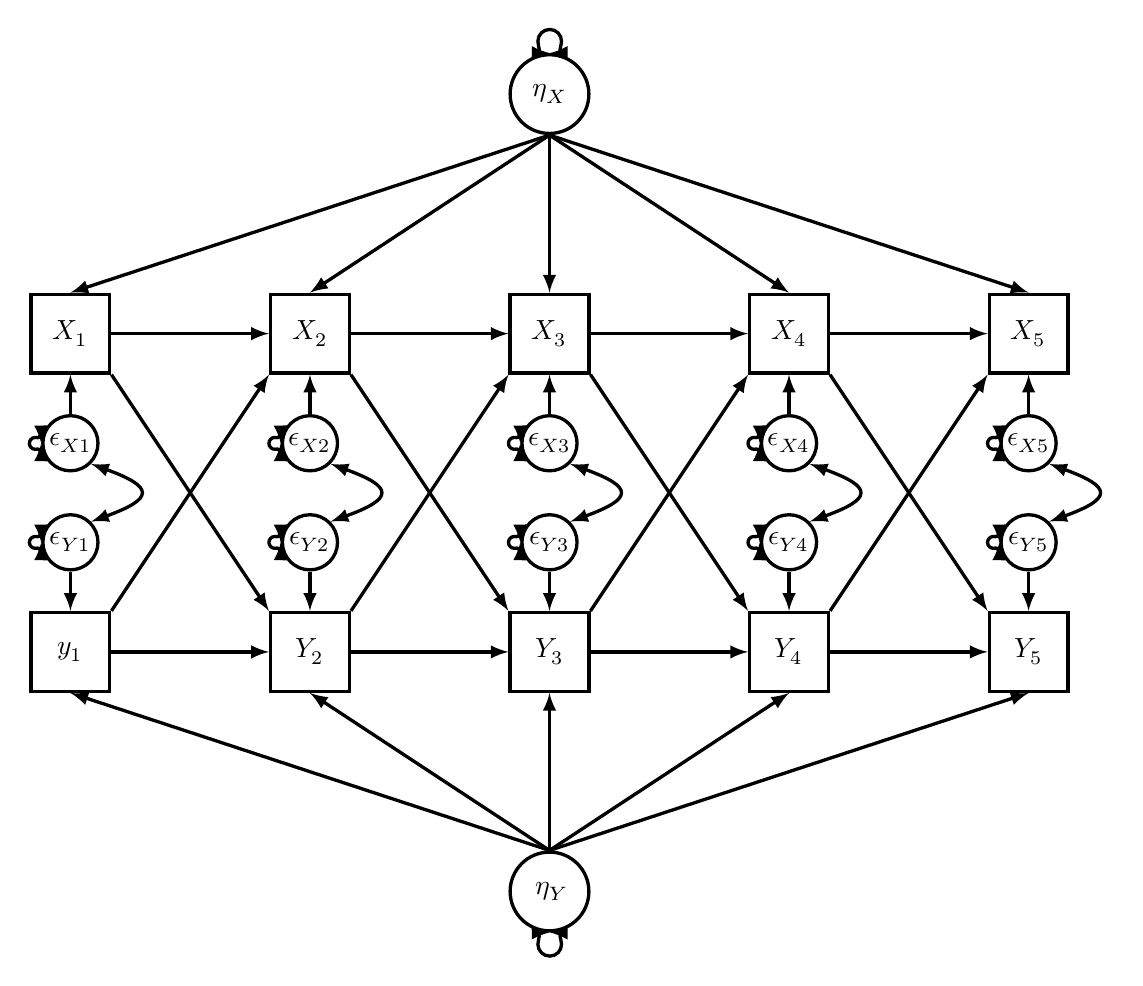
\begin{tikzpicture}[auto,node distance=.5cm, scale=0.5,
latent/.style={circle,draw,very thick,inner sep=0pt,minimum size=10mm,align=center},
manifest/.style={rectangle,draw,very thick,inner sep=0pt,minimum width=10mm,minimum height=10mm},
resid/.style={circle,draw,very thick,inner sep=0pt,minimum size=7mm,align=center},
paths/.style={->, very thick, -latex},
double/.style={very thick, latex-latex}
]
%create nodes
\node[manifest] (y1) at (0,0) {$y_1$};
\node[manifest, right=2cm of y1] (y2) {$Y_2$};
\node[manifest, right=2cm of y2] (y3){$Y_3$};
\node[manifest, right=2cm of y3] (y4){$Y_4$};
\node[manifest, right=2cm of y4] (y5){$Y_5$};

\node[manifest, above=3cm of y1] (x1){$X_1$};
\node[manifest, right=2cm of x1] (x2){$X_2$};
\node[manifest, right=2cm of x2] (x3){$X_3$};
\node[manifest, right=2cm of x3] (x4){$X_4$};
\node[manifest, right=2cm of x4] (x5){$X_5$};

\node[resid, below=0.5cm of x1] (ex1){$\epsilon_{X1}$};
\node[resid, below=0.5cm of x2] (ex2){$\epsilon_{X2}$};
\node[resid, below=0.5cm of x3] (ex3){$\epsilon_{X3}$};
\node[resid, below=0.5cm of x4] (ex4){$\epsilon_{X4}$};
\node[resid, below=0.5cm of x5] (ex5){$\epsilon_{X5}$};

\node[resid, above=0.5cm of y1] (ey1){$\epsilon_{Y1}$};
\node[resid, above=0.5cm of y2] (ey2){$\epsilon_{Y2}$};
\node[resid, above=0.5cm of y3] (ey3){$\epsilon_{Y3}$};
\node[resid, above=0.5cm of y4] (ey4){$\epsilon_{Y4}$};
\node[resid, above=0.5cm of y5] (ey5){$\epsilon_{Y5}$};

\node[latent, above=2cm of x3] (etax){$\eta_X$};
\node[latent, below=2cm of y3] (etay){$\eta_Y$};

%draw paths
\draw[paths] (ex1) -- (x1);
\draw[paths] (ex2) -- (x2);
\draw[paths] (ex3) -- (x3);
\draw[paths] (ex4) -- (x4);
\draw[paths] (ex5) -- (x5);

\draw[paths] (ey1) -- (y1);
\draw[paths] (ey2) -- (y2);
\draw[paths] (ey3) -- (y3);
\draw[paths] (ey4) -- (y4);
\draw[paths] (ey5) -- (y5);

\draw[paths] (x1.south east) -- (y2.north west);
\draw[paths] (x2.south east) -- (y3.north west);
\draw[paths] (x3.south east) -- (y4.north west);
\draw[paths] (x4.south east) -- (y5.north west);
\draw[paths] (y1.north east) -- (x2.south west);
\draw[paths] (y2.north east) -- (x3.south west);
\draw[paths] (y3.north east) -- (x4.south west);
\draw[paths] (y4.north east) -- (x5.south west);

\draw[paths] (x1.east) -- (x2.west);
\draw[paths] (x2.east) -- (x3.west);
\draw[paths] (x3.east) -- (x4.west);
\draw[paths] (x4.east) -- (x5.west);
\draw[paths] (y1.east) -- (y2.west);
\draw[paths] (y2.east) -- (y3.west);
\draw[paths] (y3.east) -- (y4.west);
\draw[paths] (y4.east) -- (y5.west);

\draw[paths] (etax.south) -- (x1.north);
\draw[paths] (etax.south) -- (x2.north);
\draw[paths] (etax.south) -- (x3.north);
\draw[paths] (etax.south) -- (x4.north);
\draw[paths] (etax.south) -- (x5.north);

\draw[paths] (etay.north) -- (y1.south);
\draw[paths] (etay.north) -- (y2.south);
\draw[paths] (etay.north) -- (y3.south);
\draw[paths] (etay.north) -- (y4.south);
\draw[paths] (etay.north) -- (y5.south);

%draw covariances of residuals
\draw[double] (ex1.south east) to [out=-20, in=20, looseness=3](ey1.north east);
\draw[double] (ex2.south east) to [out=-20, in=20, looseness=3](ey2.north east);
\draw[double] (ex3.south east) to [out=-20, in=20, looseness=3](ey3.north east);
\draw[double] (ex4.south east) to [out=-20, in=20, looseness=3](ey4.north east);
\draw[double] (ex5.south east) to [out=-20, in=20, looseness=3](ey5.north east);

%draw variance of latent factors
\draw[double] (etax.north) arc [start angle=269, end angle = -89, x radius = 0.3cm, y radius=0.3cm];
\draw[double] (etay.south) arc [start angle=-269, end angle = 89, x radius = 0.3cm, y radius=0.3cm];

%draw residual variances
\draw[double] (ex1.west) arc [start angle=1, end angle = 359, x radius = 0.15cm, y radius=0.15cm];
\draw[double] (ex2.west) arc [start angle=1, end angle = 359, x radius = 0.15cm, y radius=0.15cm];
\draw[double] (ex3.west) arc [start angle=1, end angle = 359, x radius = 0.15cm, y radius=0.15cm];
\draw[double] (ex4.west) arc [start angle=1, end angle = 359, x radius = 0.15cm, y radius=0.15cm];
\draw[double] (ex5.west) arc [start angle=1, end angle = 359, x radius = 0.15cm, y radius=0.15cm];

\draw[double] (ey1.west) arc [start angle=1, end angle = 359, x radius = 0.15cm, y radius=0.15cm];
\draw[double] (ey2.west) arc [start angle=1, end angle = 359, x radius = 0.15cm, y radius=0.15cm];
\draw[double] (ey3.west) arc [start angle=1, end angle = 359, x radius = 0.15cm, y radius=0.15cm];
\draw[double] (ey4.west) arc [start angle=1, end angle = 359, x radius = 0.15cm, y radius=0.15cm];
\draw[double] (ey5.west) arc [start angle=1, end angle = 359, x radius = 0.15cm, y radius=0.15cm];

\end{tikzpicture}}

}

\subcaption{\label{fig-anonymous-1}Dynamic Panel Model}
\end{minipage}%
%
\begin{minipage}[t]{0.50\linewidth}

{\centering 

\resizebox{!}{\linewidth}{\usetikzlibrary{positioning}
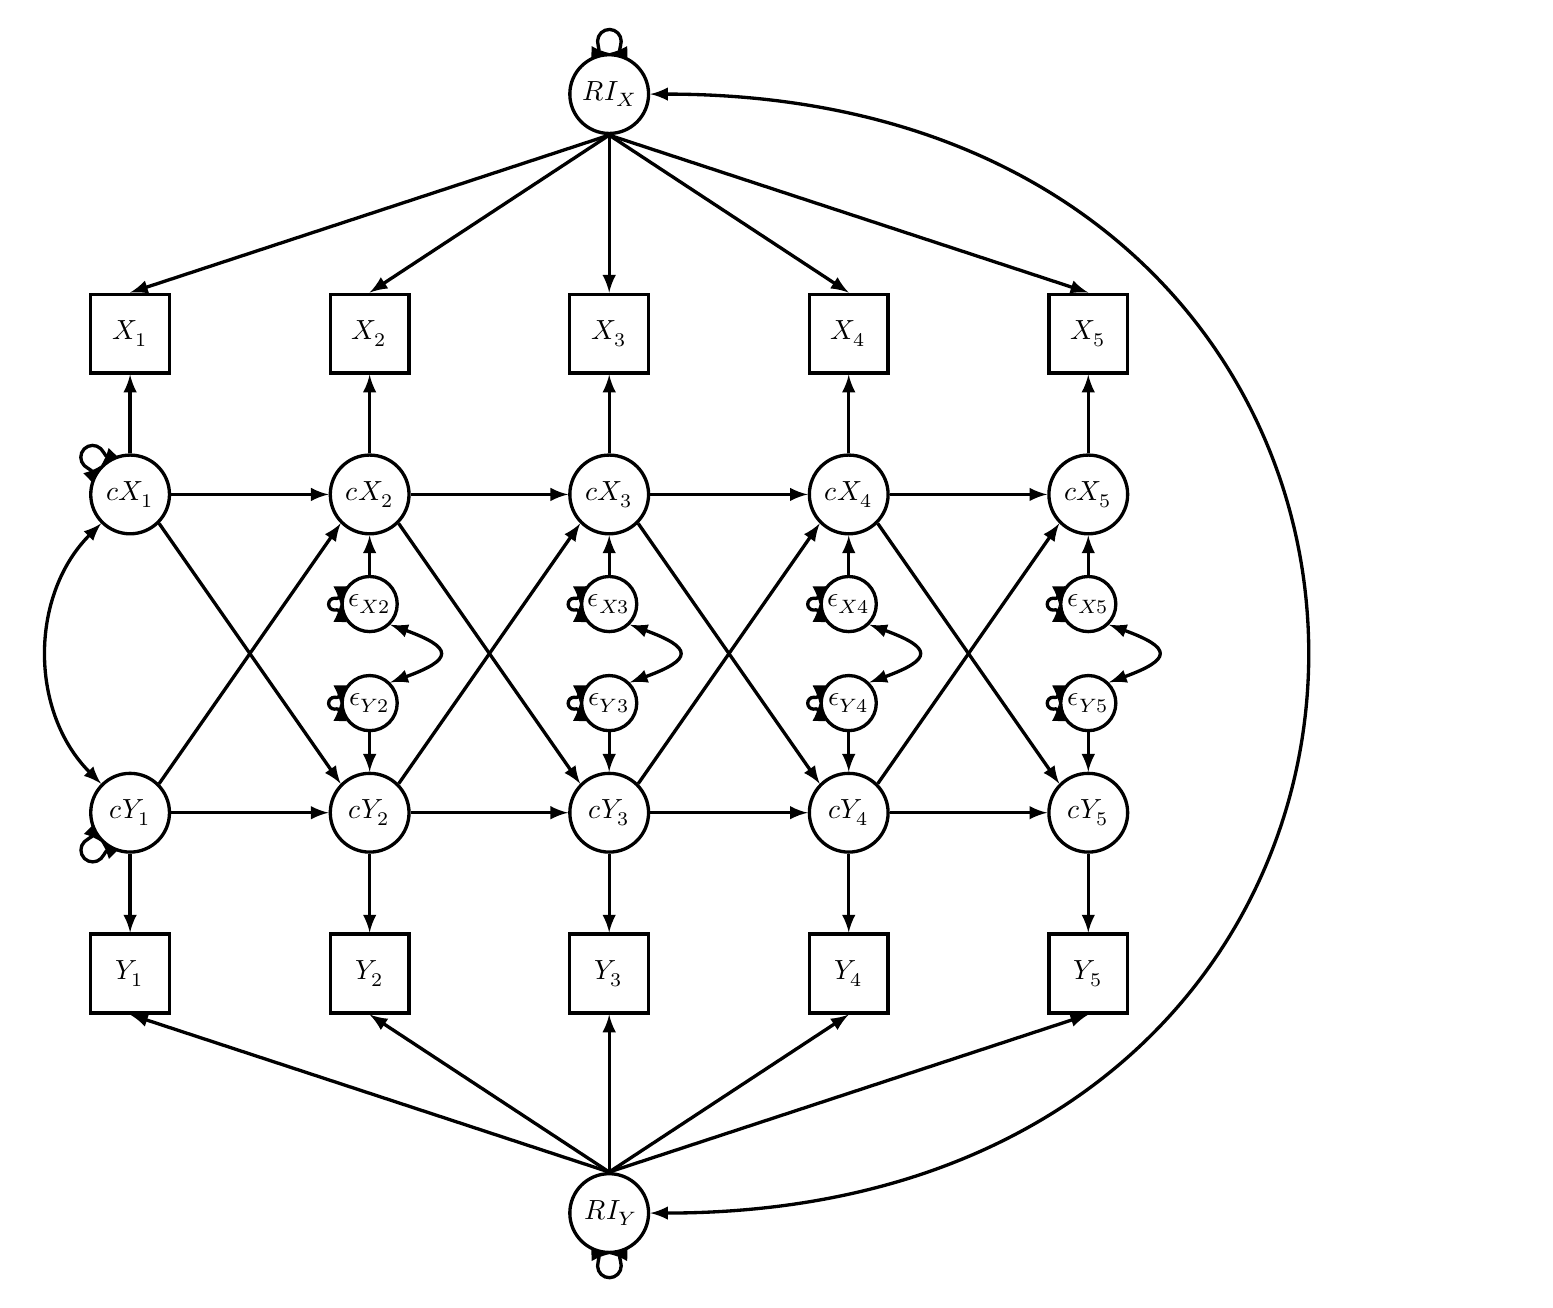
\begin{tikzpicture}[auto,node distance=.5cm, scale=0.5,
latent/.style={circle,draw,very thick,inner sep=0pt,minimum size=10mm,align=center},
manifest/.style={rectangle,draw,very thick,inner sep=0pt,minimum width=10mm,minimum height=10mm},
resid/.style={circle,draw,very thick,inner sep=0pt,minimum size=7mm,align=center},
paths/.style={->, very thick, -latex},
double/.style={very thick, latex-latex}
]
%create nodes
\node[latent] (cy1) at (0,0) {$cY_1$};
\node[latent, right=2cm of cy1] (cy2) {$cY_2$};
\node[latent, right=2cm of cy2] (cy3){$cY_3$};
\node[latent, right=2cm of cy3] (cy4){$cY_4$};
\node[latent, right=2cm of cy4] (cy5){$cY_5$};

\node[latent, above=3cm of cy1] (cx1){$cX_1$};
\node[latent, right=2cm of cx1] (cx2){$cX_2$};
\node[latent, right=2cm of cx2] (cx3){$cX_3$};
\node[latent, right=2cm of cx3] (cx4){$cX_4$};
\node[latent, right=2cm of cx4] (cx5){$cX_5$};

\node[resid, below=0.5cm of cx2] (ex2){$\epsilon_{X2}$};
\node[resid, below=0.5cm of cx3] (ex3){$\epsilon_{X3}$};
\node[resid, below=0.5cm of cx4] (ex4){$\epsilon_{X4}$};
\node[resid, below=0.5cm of cx5] (ex5){$\epsilon_{X5}$};

\node[resid, above=0.5cm of cy2] (ey2){$\epsilon_{Y2}$};
\node[resid, above=0.5cm of cy3] (ey3){$\epsilon_{Y3}$};
\node[resid, above=0.5cm of cy4] (ey4){$\epsilon_{Y4}$};
\node[resid, above=0.5cm of cy5] (ey5){$\epsilon_{Y5}$};

\node[manifest, above=1cm of cx1] (x1){$X_1$};
\node[manifest, above=1cm of cx2] (x2){$X_2$};
\node[manifest, above=1cm of cx3] (x3){$X_3$};
\node[manifest, above=1cm of cx4] (x4){$X_4$};
\node[manifest, above=1cm of cx5] (x5){$X_5$};

\node[manifest, below=1cm of cy1] (y1){$Y_1$};
\node[manifest, below=1cm of cy2] (y2){$Y_2$};
\node[manifest, below=1cm of cy3] (y3){$Y_3$};
\node[manifest, below=1cm of cy4] (y4){$Y_4$};
\node[manifest, below=1cm of cy5] (y5){$Y_5$};

\node[latent, above=2cm of x3] (etax){$RI_X$};
\node[latent, below=2cm of y3] (etay){$RI_Y$};

%observed to within paths
\draw[paths] (cx1) -- (x1);
\draw[paths] (cx2) -- (x2);
\draw[paths] (cx3) -- (x3);
\draw[paths] (cx4) -- (x4);
\draw[paths] (cx5) -- (x5);
\draw[paths] (cy1) -- (y1);
\draw[paths] (cy2) -- (y2);
\draw[paths] (cy3) -- (y3);
\draw[paths] (cy4) -- (y4);
\draw[paths] (cy5) -- (y5);

%draw paths

\draw[paths] (ex2) -- (cx2);
\draw[paths] (ex3) -- (cx3);
\draw[paths] (ex4) -- (cx4);
\draw[paths] (ex5) -- (cx5);

\draw[paths] (ey2) -- (cy2);
\draw[paths] (ey3) -- (cy3);
\draw[paths] (ey4) -- (cy4);
\draw[paths] (ey5) -- (cy5);

\draw[paths] (cx1.south east) -- (cy2.north west);
\draw[paths] (cx2.south east) -- (cy3.north west);
\draw[paths] (cx3.south east) -- (cy4.north west);
\draw[paths] (cx4.south east) -- (cy5.north west);
\draw[paths] (cy1.north east) -- (cx2.south west);
\draw[paths] (cy2.north east) -- (cx3.south west);
\draw[paths] (cy3.north east) -- (cx4.south west);
\draw[paths] (cy4.north east) -- (cx5.south west);

\draw[paths] (cx1.east) -- (cx2.west);
\draw[paths] (cx2.east) -- (cx3.west);
\draw[paths] (cx3.east) -- (cx4.west);
\draw[paths] (cx4.east) -- (cx5.west);
\draw[paths] (cy1.east) -- (cy2.west);
\draw[paths] (cy2.east) -- (cy3.west);
\draw[paths] (cy3.east) -- (cy4.west);
\draw[paths] (cy4.east) -- (cy5.west);

\draw[paths] (etax.south) -- (x1.north);
\draw[paths] (etax.south) -- (x2.north);
\draw[paths] (etax.south) -- (x3.north);
\draw[paths] (etax.south) -- (x4.north);
\draw[paths] (etax.south) -- (x5.north);

\draw[paths] (etay.north) -- (y1.south);
\draw[paths] (etay.north) -- (y2.south);
\draw[paths] (etay.north) -- (y3.south);
\draw[paths] (etay.north) -- (y4.south);
\draw[paths] (etay.north) -- (y5.south);

%draw covariances of residuals
\draw[double] (ex2.south east) to [out=-20, in=20, looseness=3](ey2.north east);
\draw[double] (ex3.south east) to [out=-20, in=20, looseness=3](ey3.north east);
\draw[double] (ex4.south east) to [out=-20, in=20, looseness=3](ey4.north east);
\draw[double] (ex5.south east) to [out=-20, in=20, looseness=3](ey5.north east);

%covariance cX1 and cY1
\draw[double](cx1.south west) to [out=225, in=135] (cy1.north west);

%draw variance of latent factors
\draw[double] (etax.north) arc [start angle=269, end angle = -89, x radius = 0.3cm, y radius=0.3cm];
\draw[double] (etay.south) arc [start angle=-269, end angle = 89, x radius = 0.3cm, y radius=0.3cm];

%draw residual variances
\draw[double] (ex2.west) arc [start angle=1, end angle = 359, x radius = 0.15cm, y radius=0.15cm];
\draw[double] (ex3.west) arc [start angle=1, end angle = 359, x radius = 0.15cm, y radius=0.15cm];
\draw[double] (ex4.west) arc [start angle=1, end angle = 359, x radius = 0.15cm, y radius=0.15cm];
\draw[double] (ex5.west) arc [start angle=1, end angle = 359, x radius = 0.15cm, y radius=0.15cm];

\draw[double] (ey2.west) arc [start angle=1, end angle = 359, x radius = 0.15cm, y radius=0.15cm];
\draw[double] (ey3.west) arc [start angle=1, end angle = 359, x radius = 0.15cm, y radius=0.15cm];
\draw[double] (ey4.west) arc [start angle=1, end angle = 359, x radius = 0.15cm, y radius=0.15cm];
\draw[double] (ey5.west) arc [start angle=1, end angle = 359, x radius = 0.15cm, y radius=0.15cm];

%draw variance cx1 and cy1
\draw[double] (cx1.north west) arc [start angle=-44, end angle = 314, x radius = 0.3cm, y radius=0.3cm];
\draw[double] (cy1.south west) arc [start angle=45, end angle = 405, x radius = 0.3cm, y radius=0.3cm];

%covariance between latent factors
\draw[double] (etax.east) to [out=0, in=0, looseness=2] (etay.east);

\end{tikzpicture}}

}

\subcaption{\label{fig-anonymous-2}RI-CLPM}
\end{minipage}%

\caption{\label{fig-models}Models}

\end{figure}

\hypertarget{discussion}{%
\section{Discussion}\label{discussion}}

\newpage{}

\hypertarget{references}{%
\section*{References}\label{references}}
\addcontentsline{toc}{section}{References}

\hypertarget{refs}{}
\begin{CSLReferences}{1}{0}
\leavevmode\vadjust pre{\hypertarget{ref-brown2021}{}}%
Brown, D. W., Greene, T. J., Swartz, M. D., Wilkinson, A. V., \&
DeSantis, S. M. (2021). Propensity score stratification methods for
continuous treatments. \emph{Statistics in Medicine}, \emph{40}(5),
1189--1203. \url{https://doi.org/10.1002/sim.8835}

\leavevmode\vadjust pre{\hypertarget{ref-ludtke2021}{}}%
Lüdtke, O., \& Robitzsch, A. (2021). \emph{A {Critique} of the {Random
Intercept Cross-Lagged Panel Model}} {[}Preprint{]}. {PsyArXiv}.
\url{https://doi.org/10.31234/osf.io/6f85c}

\leavevmode\vadjust pre{\hypertarget{ref-morris2019}{}}%
Morris, T. P., White, I. R., \& Crowther, M. J. (2019). Using simulation
studies to evaluate statistical methods. \emph{Statistics in Medicine},
\emph{38}(11), 2074--2102. \url{https://doi.org/10.1002/sim.8086}

\leavevmode\vadjust pre{\hypertarget{ref-murayama2022}{}}%
Murayama, K., \& Gfrörer, T. (2022). \emph{Thinking clearly about
time-invariant confounders in cross-lagged panel models: {A} guide for
choosing a statistical model from a causal inference perspective}
{[}Preprint{]}. {PsyArXiv}.

\leavevmode\vadjust pre{\hypertarget{ref-usami2019}{}}%
Usami, S., Murayama, K., \& Hamaker, E. L. (2019). A unified framework
of longitudinal models to examine reciprocal relations.
\emph{Psychological Methods}, \emph{24}(5), 637--657.
\url{https://doi.org/10.1037/met0000210}

\leavevmode\vadjust pre{\hypertarget{ref-vansteelandt2014}{}}%
Vansteelandt, S., \& Daniel, R. m. (2014). On regression adjustment for
the propensity score. \emph{Statistics in Medicine}, \emph{33}(23),
4053--4072. \url{https://doi.org/10.1002/sim.6207}

\end{CSLReferences}



\end{document}
